\chapter{Conditional Random Fields (\glsentryshortpl{crf})}\label{cha:crfs}

In this chapter, we give an introduction to the \glsfirst{crf} framework.
We first provide an overview of relevant concepts in probability theory and graphical models.
Following this, we will introduce the concept of \glspl{crf} and discuss the inference and learning of \gls{crf} models.

In addition to relevant definitions, we use a simplified example of the author extraction problem that we will discuss in \Cref{cha:author-extraction}.
This example is based on the set of four reference strings given in \Cref{fig:example-reference-strings}.

\begin{figure}[t]
\begin{framed}
  Mia Friedrich (2010): Title of the first example, Berlin: Springer.

M\"{u}ller, Friedrich (2010): Title of the second example, Berlin: Springer.

Max M\"{u}ller, Fritz Schmidt (2010): Friedrich in title, Berlin: Springer.

Mia Wagner, Max Friedrich Schmidt (2010): Fourth title, Berlin: Springer.

\end{framed}
\caption{Example of four reference strings.}
\label{fig:example-reference-strings}
\end{figure}
\section{Foundations}\label{sec:foundations}
\subsection{Probability Theory}\label{subsec:probability-theory}
Several concepts from probability theory are crucial for an understanding of \glspl{crf} and they all build on the notion of \glspl{probability distribution}.

A \gls{probability distribution} $P$ is defined using two sets.
The first set is the \gls{outcome space} \glssymbol{outcome space}, which contains all possible outcomes of an experiment.
The second set is called \gls{event space} \glssymbol{event space}.
It contains measurable \glspl{event} to which we can assign probabilities~\citep{koller2009probabilistic}.
Such a measurable \gls{event} $\alpha$ is a subset of \glssymbol{outcome space}: $\alpha\subseteq\glssymbol{outcome space}$.

Further, the following four properties must hold true for the \gls{event space}~\citep{koller2009probabilistic}:
\begin{itemize}
  \item It contains the \textit{empty event} which consists of the empty set $\emptyset$.
  \item It contains the \textit{trivial event} which is the set of all possible outcomes \glssymbol{outcome space}.
  \item It is closed under union: If \glspl{event} $\alpha$ and $\beta$ are in \glssymbol{event space}, then so is $\alpha\cup\beta$.
  \item It is closed under complementation: If \gls{event} $\alpha$ is in \glssymbol{event space}, then so is $\glssymbol{outcome space}\setminus\alpha$.
\end{itemize}

To describe the relation between \glssymbol{event space} and \glssymbol{outcome space}, we first define the \gls{power set}:
A \gls{power set} of a set $A$ is defined as the set of all possible subsets of $A$, including the empty set $\emptyset$ and the set $A$ itself:
\begin{equation}
  \label{equ:power-set}
  \glssymbol{power set}(A)=\left\{B\mid B\subseteq A\right\}
\end{equation}
Using this, we can define \gls{event space} \glssymbol{event space} as a subset of the \gls{power set} of the \gls{outcome space} \glssymbol{outcome space}:
\begin{equation*}
  \glssymbol{event space}\subseteq\glssymbol{power set}(\glssymbol{outcome space}).
\end{equation*}

\newpage

The \gls{probability distribution} $P$ now describes a mapping from \glspl{event} in \glssymbol{event space} to real numbers according to the following rules \citep{koller2009probabilistic}:
\begin{itemize}
  \item $P(\alpha)\geq 0 $ for all $ \alpha \in S$.
  \item $P(\glssymbol{outcome space})=1$.
  \item If $\alpha,\beta\in \glssymbol{event space}$ and $\alpha\cap\beta = \emptyset$, then $P(\alpha\cup\beta)=P(\alpha)+P(\beta)$.
\end{itemize}

To clarify this using our author extraction example, we first define the \gls{outcome space} \glssymbol{outcome space} as the set consisting of the four reference strings in \Cref{fig:example-reference-strings}.
More precisely, a reference string consists of a sequence of words ``$w_1\ w_2\ \dots\ w_N$'' where words are separated by whitespaces and where $N$ is the number of words in the sequence.
For simplicity reasons, $N$ is the same for all four reference strings in \Cref{fig:example-reference-strings}.
We now consider two \glspl{event}:
\begin{equation*}
  \begin{split}
    \mathit{firstLN}&=\left\{w_1\ \dots\ w_N \mid w_1\ \text{is a last name}\right\}.\\
    \mathit{secondEC}&=\left\{w_1\ \dots\ w_N \mid w_2\ \text{ends with a comma}\right\}.
  \end{split}
\end{equation*}
In other words, $\mathit{firstLN}$ contains all reference strings in \glssymbol{outcome space} in which the first word of the sequence is a last name and $\mathit{secondEC}$ contains all reference strings in \glssymbol{outcome space} in which the second word of the sequence ends with a comma.

To fulfill the three properties of an \gls{event space} \glssymbol{event space}, we need to introduce a number of additional \glspl{event}.
First, we add the empty \gls{event} $\emptyset$ and the trivial \gls{event} $\Omega$ to \glssymbol{event space}.
Further, to fulfill the property of \glssymbol{event space} being closed under complementation, we then add the complement of $\mathit{firstLN}$ and $\mathit{secondEC}$:
\begin{equation*}
  \begin{split}
    \mathit{firstNotLN}&=\glssymbol{outcome space}\setminus\textit{firstLN}.\\
    \mathit{secondNotEC}&=\glssymbol{outcome space}\setminus\textit{secondEC}.\\
  \end{split}
\end{equation*}
To fulfill the union property of \glssymbol{event space}, we add all unions of \glspl{event}.
Then, we again need to add the complements of the newly added union of \glspl{event}.
This repeats until all possible unions and complements are added to \glssymbol{event space}.
Even for this simple example, the resulting \gls{event space} is already considerably big.
In the following, we thereby to not explicitly discuss the content of \glssymbol{event space}.

\bigskip

We now consider the resulting \glspl{probability distribution} for this example.
Based on the four reference strings in \glssymbol{outcome space}, we assign the corresponding probabilities to the events in \glssymbol{event space}.
Examples for this are:
\begin{equation*}
    \begin{split}
      P(\mathit{firstLN})&=1/4=0.25.\\
      P(\mathit{firstNotLN})&=3/4=0.75.\\
      P(\mathit{secondEC})&=2/4=0.5.\\
      P(\mathit{secondNotEC})&=2/4=0.5.
    \end{split}
\end{equation*}
Note that, when building the sum over all assigned probabilities, we result in a number greater than $1$.
When recalling the rules for \glspl{probability distribution}, we see that the probability for the union of two \glspl{event} is only defined as the addition of their probabilities if the intersection of the two events is the empty set.
Thereby, our defined \glspl{probability distribution} remain valid.

\bigskip

Another important concept in probability theory are \glspl{random variable}.
A \gls{random variable} $X$ is a \gls{function} that associates a value with each outcome in \glssymbol{outcome space}~\cite{koller2009probabilistic}.
In addition, $\mathit{Val}(X)$ is the set of values that $X$ can take.
The elements in $\mathit{Val}(X)$ are also called \glspl{assignment} to $X$.

Following our example, we define the \gls{random variable} $LN_1$ as a \gls{function} that, given a reference string, returns the value $\mathit{true}$ if the first word in the sequence is a last name and the value $\mathit{false}$ if it does not.
This results in: $\mathit{Val}(LN_1)=\{\mathit{true}, \mathit{false}\}$.
Similarly, $EC_2$ is defined as the function that associates the value $\mathit{true}$ with a reference string if the second word ends with a comma and $\mathit{false}$ if the second word does not end with a comma.

\bigskip

Given a \gls{random variable} $X$, $P(X)$ is the \gls{probability distribution} over $\mathit{Val}(X)$~\cite{koller2009probabilistic}.
It is also referred to as the \gls{marginal distribution} over $X$.
An \gls{assignment} of a concrete value $x\in \mathit{Val}(X)$ to $X$ is denoted by $P(X=x)$ or short $P(x)$.

We can now define our \glspl{probability distribution} on \glspl{random variable} instead of \glspl{event}, for example:
\begin{equation*}
  \begin{split}
    P(\mathit{firstLN})&= P(LN_1{=}\mathit{true})\\
    P(\mathit{secondNotEC})&= P(EC_2{=}\mathit{false}).
  \end{split}
\end{equation*}

\bigskip

We now consider the concept of \gls{joint probability}.
Given two \glspl{event} $\alpha$ and $\beta$, the \gls{joint probability} $P(\alpha,\beta)$ corresponds to the probability of the intersection of the two events~\citep{teschl2007mathematik}:
\begin{equation*}
  P(\alpha,\beta)=\alpha\cap\beta.
\end{equation*}

This concept can also be applied to \glspl{random variable}.
Given \glspl{random variable} $X$ and $Y$ which are defined on the same \gls{event space} \glssymbol{event space}, we consider their \gls{joint distribution} $P(X,Y)$.
For the \glspl{assignment} $x$ and $y$, $P(X{=}x,Y{=}y)$ associates a probability with the subset of $\Omega$ which is specified by  $x$ and $y$~\citep{koller2009probabilistic}.
The \gls{joint distribution} for more than two \glspl{random variable} is defined accordingly.

In our example, $P(LN_1,EC_2)$ has the following values:
\begin{equation*}
  \begin{split}
    P(LN_1{=}\mathit{false},EC_2{=}\mathit{false})&=1/4=0.25.\\
    P(LN_1{=}\mathit{false},EC_2{=}\mathit{true})&=2/4=0.5.\\
    P(LN_1{=}\mathit{true},EC_2{=}\mathit{false})&=1/4=0.25.\\
    P(LN_1{=}\mathit{true},EC_2{=}\mathit{true})&=0/4=0.
  \end{split}
\end{equation*}

\bigskip

A notation that is frequently used in this chapter is that of a set of \glspl{random variable} $\mathbf{X}=\left\{ X_1,\dots,X_N\right\}$.
The set of \glspl{assignment} to $\mathbf{X}$ is denoted by $\mathbf{x}=\left\{ x_1,\dots,x_N\right\}$ where each $x_n$ is an \gls{assignment} to $X_n\in\mathbf{X}$.
The set of \glspl{assignment} $\mathbf{x}$ is also called a \gls{full assignment} to $\mathbf{X}$.
Any \gls{event} that is described using $\mathbf{X}$ must be a union of \glspl{full assignment} to $\mathbf{X}$.
In the following, we assume every \gls{outcome space} \glssymbol{outcome space} to be defined as a set of \glspl{full assignment} to some set of \glspl{random variable} $\mathcal{X}$.
This is also called a \gls{canonical outcome space}~\citep{koller2009probabilistic}.

We demonstrate this by extending our definitions of $LN_1$ and $EC_2$ and apply them to all words in a reference string of length $N$.
This gives us two sets of \glspl{random variable}:
\begin{equation*}
  \begin{split}
    \mathbf{LN}=& \{LN_1, \dots, LN_N\}.\\
    \mathbf{EC}=& \{EC_1, \dots, EC_N\}.
  \end{split}
\end{equation*}
Using this, we define a \gls{canonical outcome space} \glssymbol{outcome space} as the set of all \glspl{full assignment} to $\mathbf{LN}\cup\mathbf{EC}$.

\bigskip

The \gls{conditional probability} of an \gls{event} $\beta$ given an \gls{event} $\alpha$ with $P(\alpha)>0$ is defined as~\cite{koller2009probabilistic}:

\begin{equation}
\label{equ:conditional-probability-event}
P(\beta\mid\alpha) = \frac{P(\alpha\cap\beta)}{P(\alpha)}.
\end{equation}
This definition can be extended to \glspl{random variable}.
Given that the probability for every \gls{assignment} to $X$ is greater than zero, the \gls{cpd}\glsunset{conditional probability distribution} $P(Y\mid X)$ is calculated with
\begin{equation}
\label{equ:conditional-probability-random-variable-1}
P(Y\mid X) = \frac{P(X,Y)}{P(X)}
\end{equation}
and for sets of \glspl{random variable} $\mathbf{X}$ and $\mathbf{Y}$ we have:
\begin{equation}
\label{equ:conditional-probability-random-variable-2}
P(\mathbf{Y}\mid \mathbf{X}) = \frac{P(\mathbf{X},\mathbf{Y})}{P(\mathbf{X})}.
\end{equation}

Again taking the reference strings in \Cref{fig:example-reference-strings}, we have for example:
\begin{equation*}
  P(EC_2{=}\mathit{true}\mid LN_1{=}\mathit{false})=\frac{P(LN_1{=}\mathit{false}, EC_2{=}\mathit{true})}{P(LN_1{=}\mathit{false})}=\frac{0.5}{0.75}\approx0.6667.
\end{equation*}

\bigskip

A value that can be used as a metric for comparing different \glspl{probability distribution} with each other is called \gls{expectation}.
Given a discrete \gls{random variable} $X$, we define the expectation $E[X]$ of $X$ under the distribution $P$ as~\cite{koller2009probabilistic}:
\begin{equation}
  \label{equ:expectation-x-1}
  E[X]=\sum_{x\in \mathit{Val}(X)} x\cdot P(x).
\end{equation}

To apply this definition to our example, we redefine $\mathit{Val}(LN_1)=\{\mathit{true},\mathit{false}\}$ as $\mathit{Val}(LN_1)=\{1,0\}$ where we replace $\mathit{true}$ and $\mathit{false}$ with the values $1$ and $0$, respectively.
This gives us:
\begin{equation*}
  \begin{split}
  \label{equ:expectation-x-2}
  E[LN_1]&=\sum_{x\in \mathit{Val}(LN_1)} x\cdot P(x)\\
  &=1\cdot P(LN_1{=}1)+0\cdot P(LN_1{=}0)\\
  &=1\cdot 0.25+0\cdot 0.75\\
  &=0.25.
  \end{split}
\end{equation*}

\subsection{Probabilistic Graphical Models}\label{subsec:graphical-models}
When encoding practical problems with \glspl{probability distribution}, a key insight is that \glspl{random variable} often only interact with a low number of other \glspl{random variable}~\citep{koller2009probabilistic}.
This makes it possible to represent such distributions as graphs in a tractable and transparent way, allowing domain experts to evaluate their properties~\citep{koller2009probabilistic}.
\Glspl{probabilistic graphical model} are such representations.

\bigskip

In a \gls{probabilistic graphical model}, \glspl{node} represent the elements from the set of \glspl{random variable} $\mathcal{X}$ of a \gls{probability distribution}.
An \gls{edge} then denotes a probabilistic interaction between its two incident \glspl{node}~\citep{koller2009probabilistic}.

There are two fundamental groups of graphical models, based on the type of edge that are used: \glspl{bayesian network} and \glspl{markov network}.
Both models have in common that their set of \glspl{random variable} $\mathcal{X}$ can be separated into two subsets:
$\mathbf{X}$ contains the so-called \glspl{observed variable} which usually represent specific features of the input.
$\mathbf{Y}$ contains the \glspl{target variable} which we usually want to infer using a graphical model.
We thereby have $\mathcal{X}=\{\mathbf{X}\cup\mathbf{Y}\}$ with $\mathbf{X}\cap\mathbf{Y}=\emptyset$.
Yet, there are fundamental differences between \glspl{bayesian network} and \glspl{markov network}.
In the following, we use our previously discussed author extraction example and define $\mathcal{X}=\{EC_2,LN_1,LN_2\}$ with $\mathbf{X}=\{EC_2\}$ and $\mathbf{Y}=\{LN_1,LN_2\}$.


\bigskip

\Glspl{bayesian network}, usually denoted by $\mathcal{G}$, are encoded using directed \glspl{edge} to build a directed acyclic graph~\citep{koller2009probabilistic}.
Considering a graphical model that is based on a \gls{bayesian network}, an \glspl{edge} from \gls{random variable} $A$ to \gls{random variable} $B$ models a probabilistic influence of $A$ on $B$.
Since the graph is acyclic and due to the directed probabilistic influences, it is possible to represent the \gls{joint distribution} $P(\mathbf{X},\mathbf{Y})$ as a product of \glspl{marginal distribution} and \glspl{cpd}~\citep{sutton2010introduction}.
We refer to \citet{koller2009probabilistic} for a detailed introduction to \glspl{bayesian network}.

\Cref{fig:example-networks} shows a \gls{bayesian network} for our author extraction example using the above defined set of \glspl{random variable} $\mathcal{X}$.
\begin{figure}[t]
\centering
\newcommand{\factorgraphnodes}{%
  \node[latent] (ln) {$LN_1$}; %
  \node[latent, right=2.4cm of ln] (fn) {$FN_2$}; %
  \node[obs, below=2.4cm of fn] (ec) {$EC_2$}; %
}
\begin{tabular}{c@{\hskip 0.75cm}c}
\begin{tikzpicture}
  \factorgraphnodes

  \edge[] {ln} {fn};
  \edge[] {fn} {ec};
  \edge[] {ln} {ec};
\end{tikzpicture}
&
\begin{tikzpicture}
  \factorgraphnodes

  \edge[-] {ln} {fn};
  \edge[-] {fn} {ec};
  \edge[-] {ln} {ec};
\end{tikzpicture}
\\
(a)& (b)\\
\end{tabular}

\caption[Two networks for $\mathcal{X}=\{EC_2,LN_1,LN_2\}$]{%
  Two networks for $\mathcal{X}=\{EC_2,LN_1,LN_2\}$:
  (a) A \gls{bayesian network} and (b) A \gls{markov network}.
}
\label{fig:example-networks}
\end{figure}
The gray node represents an \gls{observed variable} and the white nodes represent \glspl{target variable}.
From this we can derive the following \gls{joint distribution}:
\begin{equation*}
  P(EC_2,LN_1,LN_2)=P(LN_1)P(LN_2|LN_1)P(EC_2\mid LN_1,LN_2).
\end{equation*}

\bigskip

\Glspl{markov network}, usually denoted by $\mathcal{H}$, use undirected \glspl{edge} to model a symmetrical influence between two \glspl{random variable}.
Because of this, it is not possible to separate the \gls{joint distribution} $P(\mathcal{X})$ into \glspl{marginal distribution} and \glspl{cpd}.
Instead, $\mathcal{H}$ is parameterized by a set of \glspl{factor}.
A \gls{factor} $\Psi(\mathbf{D})$ is a function from a set of \glspl{random variable} $\mathbf{D}$ to $\realnumbers$~\citep{koller2009probabilistic}.
It is called nonnegative if all its entries are nonnegative.
In the following, we will consider all factors to be nonnegative.
$\mathbf{D}$ is called the \glslink{factor scope}{scope} of $\Psi$, as denoted by $Scope[\Psi]$~\citep{koller2009probabilistic}.

Using the set of \glspl{random variable} $\mathcal{X}$, we define the three factors in \Cref{tab:example-factors}: $\Psi(LN_1,EC_2)$, $\Psi(LN_2,EC_2)$, and $\Psi(LN_1,LN_2)$.
The values for the factors are calculated in the following way:
For every reference string in \Cref{fig:example-reference-strings}, which follows the given \glspl{assignment} to a \gls{factor}, we add $10$ to the corresponding factor value.
The number $10$ is chosen arbitrarily and, in a practical use case, determining this number is part of the learning process (see \Cref{sec:learning-crfs}).
As an example, for three of the four reference strings in \Cref{fig:example-reference-strings} we have $LN_1=\mathit{false}$ and $LN_2=\mathit{true}$.
Thereby, $\Psi(LN_1=\mathit{false},LN_2=\mathit{true})=30$.
If, on the other hand, no reference string agrees with the \glspl{assignment}, we set the factor value to $1$.
This value, again, is chosen arbitrarily.
The \gls{markov network} that results from the three \glspl{factor} is shown in \Cref{fig:example-networks}.
Again, the gray \gls{node} marks an \gls{observed variable} and white \glspl{node} mark \glspl{target variable}.

\begin{table}[t]
\begin{minipage}{0.5\linewidth}
\centering
$\Psi(LN_1,EC_2)$\par
\smallskip
\begin{tabular}{c c c}
 \toprule
 $LN_1$ & $EC_2$ & Value \\
 \midrule
 $\mathit{false}$ & $\mathit{false}$ & $10$ \\
 $\mathit{false}$ & $\mathit{true}$ & $20$ \\
 $\mathit{true}$ & $\mathit{false}$ & $10$ \\
 $\mathit{true}$ & $\mathit{true}$ & $1$ \\
 \bottomrule
\end{tabular}
\end{minipage}
\hfill
\begin{minipage}{0.5\linewidth}
\centering
$\Psi(LN_2,EC_2)$\par
\smallskip
\begin{tabular}{c c c}
 \toprule
 $LN_2$ & $EC_2$ & Value \\
 \midrule
 $\mathit{false}$ & $\mathit{false}$ & $10$ \\
 $\mathit{false}$ & $\mathit{true}$ & $1$ \\
 $\mathit{true}$ & $\mathit{false}$ & $10$ \\
 $\mathit{true}$ & $\mathit{true}$ & $20$ \\
 \bottomrule
\end{tabular}
\end{minipage}
\medskip
\begin{center}
$\Psi(LN_1,LN_2)$\par
\smallskip
\begin{tabular}{c c c}
 \toprule
 $LN_1$ & $LN_2$ & Value \\
 \midrule
 $\mathit{false}$ & $\mathit{false}$ & $1$ \\
 $\mathit{false}$ & $\mathit{true}$ & $30$ \\
 $\mathit{true}$ & $\mathit{false}$ & $10$ \\
 $\mathit{true}$ & $\mathit{true}$ & $1$ \\
 \bottomrule
\end{tabular}
\end{center}
\caption{Three factors for the author extraction example.}
\label{tab:example-factors}
\end{table}

\bigskip

An important operation on factors is the \gls{factor product}.
Given three disjoint sets of \glspl{assignment} $\left\{\mathbf{X}, \mathbf{Y}, \mathbf{Z}\right\}$, a \gls{factor product} $\Psi_1\times\Psi_2$ of the two factors $\Psi_1(\mathbf{X},\mathbf{Y})$ and $\Psi_2(\mathbf{Y},\mathbf{Z})$ is a factor $\Psi(\mathbf{X},\mathbf{Y},\mathbf{Z})$~\citep{koller2009probabilistic}.
The intuition is that the two factors are multiplied by aligning their common set of \glspl{random variable} $\mathbf{Y}$.

One way of calculating the \gls{factor product} of the three \glspl{factor} in \Cref{tab:example-factors} is the following:
\begin{equation*}
  \begin{split}
  &\Psi(LN_1,EC_2)\times\Psi(LN_2,EC_2)\Psi(LN_1,LN_2)\\
  &\hspace{4em}=\Psi(LN_1,LN_2,EC_2)\times\Psi(LN_1,LN_2)\\
  &\hspace{4em}=\Psi(LN_1,LN_2,EC_2).
  \end{split}
\end{equation*}
Note that in general the $\Psi(LN_1,LN_2,EC_2)$ in line two and three are not the same.
The concrete values for $\Psi(LN_1,LN_2,EC_2)$ are shown in \Cref{tab:example-factor-product}.
This demonstrates why the values in \Cref{tab:example-factors} are greater than $0$.
If a value would be $0$, all factor products involving it would also be $0$.

\bigskip

Using the definition of a \gls{factor product}, we can now define an undirected parameterization of a \gls{probability distribution}, called \gls{gibbs distribution}.
A \gls{probability distribution} $P(X_1,\dots,X_N)$ is a \gls{gibbs distribution} parameterized by a set of \glspl{factor} $\{\Psi_1(\mathbf{D}_1),\dots,\Psi_K(\mathbf{D}_K)\}$ if it is defined as~\citep{koller2009probabilistic}:
\begin{equation}
  \label{equ:gibbs-distribution}
  \begin{split}
  P\left(X_1,\dots,X_N\right) & =\frac{1}{Z}\tilde{P}\left(X_1,\dots,X_N\right) \\
  \tilde{P}\left(X_1,\dots,X_N\right) & =\prod_{k=1}^{K}\Psi_k\left(\mathbf{D}_k\right) \\
  Z & =\sum_{X_1,\ldots,X_N}\tilde{P}\left(X_1,\dots,X_N\right).
  \end{split}
\end{equation}
Here, $\tilde{P}(X_1,\dots,X_N)$ is an unnormalized measure and $Z$ is a \gls{normalizing constant}, sometimes called the \gls{partitioning function}.
It guarantees that the \gls{probability distribution} sums to $1$.
Having a \gls{gibbs distribution} $P$ where each $\mathbf{D}_k$, $1\leq k \leq K$ is a complete subgraph of a \gls{markov network} $\mathcal{H}$, we say that $P$ factorizes over $\mathcal{H}$~\citep{koller2009probabilistic}.

Based on the two \glspl{factor} from \Cref{tab:example-factors}, we now use \Cref{equ:gibbs-distribution} to calculate $P(EC_2=\mathit{false},LN_2=\mathit{false},LN_1=\mathit{true})\approx 0.2976$ (see \cref{app:subsec-gd-example-calculation}).
For the full distribution $P(EC_2,LN_2,LN_1)$ see \cref{app:subsec-gd-full-distribution}.

\bigskip

An intuition could be that \glspl{factor} are assigned to the edges of a \gls{markov network} in order to parameterize it.
Yet, such an \gls{assignment} is only able to capture the pairwise interactions between the two incident nodes~\citep{koller2009probabilistic}.
In order to model more complex interactions involving multiple nodes, a \gls{factor scope} needs to allow an arbitrary subset of nodes in $H$.
Since a factor can be assigned to an arbitrary number of nodes, visualizing \glspl{markov network} by only displaying the random variables as nodes and pairwise interactions as edges is not sufficient.
Instead, a \gls{factor graph} can be used.
A \gls{factor graph} $\mathcal{F}$ contains two types of \glspl{node}: Oval \glspl{node} to represent \glspl{random variable} and squared \glspl{node} to represent \glspl{factor}~\citep{koller2009probabilistic}.
Each factor node is associated with exactly one \gls{factor} $\Psi$ and each variable node is associated with exactly one \gls{random variable}.
The graph only contains undirected edges between factor nodes and variable nodes.
The scope of $\Psi$ is the set of variables that are adjacent to its corresponding factor node~\citep{koller2009probabilistic}.

To demonstrate the necessity of such a notation, we consider two different \glspl{factor graph} in \Cref{fig:example-factor-graphs} and their underlying \gls{markov network}.
\Gls{factor graph} (a) contains the three factors from \Cref{tab:example-factors}.
By taking the \gls{factor product} of these three \glspl{factor} we construct \gls{factor graph} (b).
When analyzing the pairwise interactions between the nodes via the given \glspl{factor}, we can see that both (a) and (b) are based on the \gls{markov network} shown in  \Cref{fig:example-networks}.

\begin{figure}[t]
\centering
%\resizebox{\linewidth}{!}{%
  \newcommand{\factorgraphnodes}{%
  \node[latent] (ln) {$LN_1$}; %
  \node[latent, right=2.4cm of ln] (fn) {$FN_2$}; %
  \node[obs, below=2.4cm of fn] (ec) {$EC_2$}; %
}
\begin{tabular}{c@{\hskip 0.75cm}c}
\begin{tikzpicture}
  \factorgraphnodes

  \factor[right=1.1cm of ln] {fn-ln-f} {above:$\Psi(LN_1,FN_2)$} {} {}; %
  \factor[above=1.9cm of ec] {ec-fn-f} {left:$\Psi(FN_2,EC_2)$} {} {}; %
  \factor[above=0.3cm of ec,xshift=-0.8215cm] {ec-ln-f} {left:$\Psi(LN_1,EC_2)$} {} {}; %
  \edge[-] {fn} {ln};
  \edge[-] {fn} {ec};
  \edge[-] {ln} {ec};
\end{tikzpicture}
&
\begin{tikzpicture}
  \factorgraphnodes

  \factor[above=1.6cm of ec,xshift=-1.2cm] {ec-fn-f} {left:$\Psi(LN_1,FN_2,EC_2)$} {} {}; %
  \edge[-] {fn} {ec-fn-f};
  \edge[-] {ln} {ec-fn-f};
  \edge[-] {ec} {ec-fn-f};
\end{tikzpicture}
\\
(a)& (b)\\
\end{tabular}

%}
\caption[Two factor graphs resulting in the same Markov network]{%
  Two \glspl{factor graph}, both resulting in the \gls{markov network} in \Cref{fig:example-networks}:
  (a) \Gls{factor graph} with three \glspl{factor}.
  (b) \Gls{factor graph} with one \gls{factor}.
  (cf. \citep{koller2009probabilistic})
}
\label{fig:example-factor-graphs}
\end{figure}

\bigskip

As stated before, a graph $\mathcal{H}$ is parameterized by a set of \glspl{factor}.
Another way to parameterize $\mathcal{H}$ is by converting the set of \glspl{factor} into the log-space~\citep{koller2009probabilistic}.
We can rewrite a factor $\Psi(\mathbf{D})$ as
\begin{equation*}
  \label{equ:energy-function}
  \Psi(\mathbf{D}) = \exp(-\epsilon(\mathbf{D}))
\end{equation*}
where $\epsilon(\mathbf{D})=-\ln\Psi(\mathbf{D})$ is called \gls{energy function}~\citep{koller2009probabilistic}.

Being in the log-space, the \gls{probability distribution} over a set of \glspl{random variable} is proportional to the exponential of the sum of its energy functions~\citep{koller2009probabilistic}:
\begin{equation}
  \label{equ:p-energy-function}
  P\left(X_1,\dots,X_N\right) \propto \exp\left\{-\sum_{k=1}^K\epsilon_k\left(\mathbf{D}_k\right)\right\}.
\end{equation}

In \Cref{tab:example-energy-functions} we apply the \gls{energy function} to the three factors in \Cref{tab:example-factors}.
As we can see, values that were $1$ in \Cref{tab:example-factors} are now $0$.

\begin{table}[t]
\begin{minipage}{0.5\linewidth}
\centering
$\epsilon(LN_1,EC_2)$\par
\smallskip
\begin{tabular}{c c l}
 \toprule
 $LN_1$ & $EC_2$ & \multicolumn{1}{c}{Value} \\
 \midrule
 $\mathit{false}$ & $\mathit{false}$ & $-\ln(10)\approx-2.3026$ \\
 $\mathit{false}$ & $\mathit{true}$ & $-\ln(20)\approx-2.9957$ \\
 $\mathit{true}$ & $\mathit{false}$ & $-\ln(10)\approx-2.3026$ \\
 $\mathit{true}$ & $\mathit{true}$ & $-\ln(1)\ \ =\ \ \ 0$ \\
 \bottomrule
\end{tabular}
\end{minipage}
\hfill
\begin{minipage}{0.5\linewidth}
\centering
$\epsilon(LN_2,EC_2)$\par
\smallskip
\begin{tabular}{c c l}
 \toprule
 $LN_2$ & $EC_2$ & \multicolumn{1}{c}{Value} \\
 \midrule
 $\mathit{false}$ & $\mathit{false}$ & $-\ln(10)\approx-2.3026$ \\
 $\mathit{false}$ & $\mathit{true}$ & $-\ln(1)\ \ = \ \ \ 0$ \\
 $\mathit{true}$ & $\mathit{false}$ & $-\ln(10)\approx-2.3026$ \\
 $\mathit{true}$ & $\mathit{true}$ & $-\ln(20)\approx-2.9957$ \\
 \bottomrule
\end{tabular}
\end{minipage}
\medskip
\begin{center}
$\epsilon(LN_1,LN_2)$\par
\smallskip
\begin{tabular}{c c l}
 \toprule
 $LN_1$ & $LN_2$ & \multicolumn{1}{c}{Value} \\
 \midrule
 $\mathit{false}$ & $\mathit{false}$ & $-\ln(1)\ \ =\ \ \ 0$ \\
 $\mathit{false}$ & $\mathit{true}$ & $-\ln(30)\approx-3.4012$ \\
 $\mathit{true}$ & $\mathit{false}$ & $-\ln(10)\approx-2.3026$ \\
 $\mathit{true}$ & $\mathit{true}$ & $-\ln(1)\ \ =\ \ \ 0$ \\
 \bottomrule
\end{tabular}
\end{center}
\caption{\Glspl{energy function} for the \glspl{factor} in \Cref{tab:example-factors}.}
\label{tab:example-energy-functions}
\end{table}

\bigskip

Using the fact that in practice many values of an \gls{energy function} $\epsilon(\mathbf{D})$ are $0$, it is possible to represent its information in a more compact way.
This is done using a number of \glspl{feature function} $f(\mathbf{D})$ and the same number of weights $\theta$.

For example, we can represent $\epsilon(LN_1,LN_2)$ from \Cref{tab:example-energy-functions} as the sum over the two indicator functions
\begin{equation*}
  \begin{split}
    f_1(LN_2,LN_1)&=\identityfun\left\{LN_2{=}\mathit{true},LN_1{=}\mathit{false}\right\}\\
    f_2(LN_2,LN_1)&=\identityfun\left\{LN_2{=}\mathit{false},LN_1{=}\mathit{true}\right\}
  \end{split}
\end{equation*}
which are multiplied with the weights $\theta_1{=}-\ln(30)$ and $\theta_2{=}-\ln(10)$:
\begin{equation*}
  \epsilon\left(LN_2,LN_1\right)=\left(-\ln(30)\cdot f_1(LN_2,LN_1)\right)+\left(-\ln(10)\cdot f_2(LN_2,LN_1)\right).
\end{equation*}
Given the \glspl{assignment} $LN_2{=}\mathit{false}$ and $LN_1{=}\mathit{true}$, we have:
\begin{equation*}
  \begin{split}
  \epsilon\left(LN_2{=}\mathit{false},LN_1{=}\mathit{true}\right)&=\left(-\ln(30)\cdot f_1(LN_2{=}\mathit{false},LN_1{=}\mathit{true})\right)\\
  &\hspace{4em}+\left(-\ln(10)\cdot f_2(LN_2{=}\mathit{false},LN_1{=}\mathit{true})\right)\\
  &=\left(-\ln(30)\cdot 0\right)+\left(-\ln(10)\cdot 1\right)\\
  &=-\ln(10).
  \end{split}
\end{equation*}

\bigskip

Based on \Cref{equ:p-energy-function}, we can now define a \gls{probability distribution} $P$ over $\mathcal{H}$ as
\begin{equation}
  \label{equ:log-linear-model}
  P\left(X_1,\dots,X_N\right) = \frac{1}{Z}\exp\left\{-\sum_{k=1}^K \theta_k f_k\left(\mathbf{D}_k\right)\right\}
\end{equation}
where $\theta_1,\dots,\theta_K$ are weights and $f_1(\mathbf{D}_1),\dots,f_K(\mathbf{D}_K)$ are \glspl{feature function} with each $\mathbf{D}_k$ being a complete subgraph in $\mathcal{H}$~\citep{koller2009probabilistic}.
Note that $K$ in \Cref{equ:log-linear-model} does not have to be equal to $K$ in \Cref{equ:p-energy-function}.
This \gls{probability distribution} is called a \gls{log-linear model}.

\bigskip

In addition to \glspl{bayesian network} and \glspl{markov network} we can further distinguish between \glspl{generative model} and \glspl{discriminative model}.
Given a set of \glspl{observed variable} $\mathbf{X}$ and a set of \glspl{target variable} $\mathbf{Y}$ with $\mathbf{X}\cap\mathbf{Y}=\emptyset$, a \gls{generative model} encodes the \gls{joint distribution} $P(\mathbf{Y},\mathbf{X})$.
A \gls{discriminative model}, on the other hand, encodes the \gls{conditional probability distribution} $P(\mathbf{Y}|\mathbf{X})$~\citep{koller2009probabilistic}.
More precisely, for a \gls{generative model} we have $P(\mathbf{Y},\mathbf{X})=P(\mathbf{Y})P(\mathbf{X}|\mathbf{Y})$.
We thereby consider how the output of the model is generated as a function of the input~\citep{sutton2010introduction}.
This leads to the main difference between the two models, namely that for a \gls{discriminative model} we do not need to model $P(\mathbf{X})$.
\citet{sutton2010introduction} argue that indeed the modeling of $P(\mathbf{X})$ in \glspl{generative model} leads to a number of difficulties and limitations.
According to them, $P(\mathbf{X})$ often contains a number of highly dependent features which restrict the modeling.
For example, in \gls{nlp} tasks, we often model word-identities as features.
Having a limited training set, we frequently have words that were unseen during training.
In order to still give a reasonable classification for unseen words, it would be beneficial to also include other features in addition to just the word-identities~\citep{sutton2010introduction}.
As an example, such features could encode whether a word is capitalized or if it appears in a name dictionary.
However, such features are highly dependent on each other.
Moreover, their dependencies would need to be represented in a \gls{generative model} which is often intractable in practice~\citep{sutton2010introduction}.
\Glspl{discriminative model} on the other hand can leverage such a combination of features despite their high dependencies since $P(\mathbf{X})$ is not modeled~\citep{koller2009probabilistic}.

Since, in \glspl{generative model}, $P(\mathbf{Y})$ is a \gls{prior distribution} and $P(\mathbf{X}|\mathbf{Y})$ a \gls{cpd}, \citet{sutton2010introduction} argue that these are more naturally modeled by the directed \gls{bayesian network}.
Consequently, because there is no \gls{prior distribution} in \glspl{discriminative model}, it is argued that they are more naturally modeled by a \gls{markov network}~\citep{sutton2010introduction}.

\bigskip

After introducing some of the fundamental concepts we will now discuss \glspl{crf}. In the following sections we will address how to encode, inference, and learn them.

\section{Encoding of \glsentryshortpl{crf}}\label{sec:definition-crfs}
A popular framework for building \glspl{probabilistic graphical model} is \acrfullpl{crf}.
Proposed by \citet{lafferty2001conditional}, the initial goal was the segmentation and labeling of sequential data.
A main motivation for \glspl{crf} is to overcome a label bias problem that other discriminative \glspl{markov network} such as \glspl{memm} tend to have~\citep{lafferty2001conditional}.\
\citet{lafferty2001conditional} argue that this is due to the per-state models which are used in models such as \glspl{memm} to represent \glspl{conditional probability}.
This can lead to a bias towards states which have fewer outgoing transitions~\citep{lafferty2001conditional}.
In order to overcome this bias, \glspl{crf} do not have per-state models but instead contain a single model to represent the \gls{joint distribution} of a set of \glspl{target variable} given a set of \glspl{observed variable}~\citep{lafferty2001conditional}.

\bigskip

\Glspl{crf} encode the \gls{conditional probability distribution} $P(\mathbf{Y}|\mathbf{X})$ where $\mathbf{Y}$ is a set of \glspl{target variable} and $\mathbf{X}$ is a set of \glspl{observed variable} with $\mathbf{Y}\cap\mathbf{X}=\emptyset$.
A \gls{crf} is constructed using a \gls{markov network} $\mathcal{H}$ where the nodes correspond to $\mathbf{Y}\cup\mathbf{X}$ and the undirected edges model a symmetrical influence between the nodes (see \Cref{subsec:graphical-models})~\citep{koller2009probabilistic}.
Given a set of \glspl{factor} $\{\Psi_1(\mathbf{D}_1),\dots\Psi_K(\mathbf{D}_K)\}$ that factorize over $\mathcal{H}$, a \gls{crf} defines $P(\mathbf{Y}\mid\mathbf{X})$ as~\citep{koller2009probabilistic}:
\begin{equation}
  \label{equ:crf-factor}
  \begin{split}
    P(\mathbf{Y}\mid\mathbf{X}) & = \frac{1}{Z(\mathbf{X})}\tilde{P}(\mathbf{Y},\mathbf{X}) \\
    \tilde{P}(\mathbf{Y},\mathbf{X}) &= \prod_{k=1}^{K}\Psi_k\left(\mathbf{D}_k\right) \\
    Z(\mathbf{X}) & = \sum_{\mathbf{Y}}\tilde{P}(\mathbf{Y},\mathbf{X}).
  \end{split}
\end{equation}
Here, similar to the \gls{gibbs distribution} in \Cref{equ:gibbs-distribution}, $\tilde{P}(\mathbf{Y},\mathbf{X})$ is the unnormalized measure and $Z(\mathbf{X})$ is a \gls{normalizing constant}~\citep{koller2009probabilistic}.
Additionally, we have that $\mathbf{D}_k\subseteq\mathbf{X}\cup\mathbf{Y}$ and $\mathbf{D}_k\not\subseteq\mathbf{X}$.
In other words, $\mathbf{D}_k$ needs to contain at least one $Y_n\in \mathbf{Y}$.

In \Cref{app:subsec-gd-example-calculation} we demonstrate that in the case of $\mathbf{D}_k\subseteq \mathbf{X}$ the term $\Psi_k(\mathbf{D}_k)$ ``cancels out'' during the calculation of $P(\mathbf{Y}\mid\mathbf{X})$.

This behavior for a $\mathbf{D}_k\subseteq\mathbf{X}$ is the result of the only difference between the definition of a \gls{gibbs distribution} in \Cref{equ:gibbs-distribution} and the definition of a \gls{crf} above, namely how the \gls{normalizing constant} $Z$ is defined~\citep{koller2009probabilistic}.
In \Cref{equ:gibbs-distribution}, $Z$ normalizes $\tilde{P}(X_1,\dots,X_N)$ with a sum over all $X_1,\dots,X_N$ resulting in a \gls{joint distribution} $P(X_1,\dots,X_N)$.
However, in \Cref{equ:crf-factor}, $Z(\mathbf{X})$ normalizes $\tilde{P}(\mathbf{Y},\mathbf{X})$ with respect to the given $\mathbf{X}$.
This way of normalizing results in the \gls{conditional probability distribution} $P(\mathbf{Y}\mid\mathbf{X})$ (cf. \Cref{equ:conditional-probability-random-variable-2}).

\Cref{app:subsec-crf-example-calculation} contains $P(LN_1{=}\mathit{true},LN_2{=}\mathit{false}\mid EC_2{=}\mathit{false})$ as an exemplary calculation according to the \glspl{factor} in \Cref{tab:example-factors}.

\bigskip

Using \Cref{equ:log-linear-model}, we can reformulate the definition of \glspl{crf} in \Cref{equ:crf-factor} as a \gls{log-linear model}:
\begin{equation}
  \label{equ:crf-log-linear}
  \begin{split}
    P(\mathbf{Y}\mid\mathbf{X}) & = \frac{1}{Z(\mathbf{X})}\tilde{P}(\mathbf{Y},\mathbf{X}) \\
    \tilde{P}(\mathbf{Y},\mathbf{X}) & = \exp\left\{ -\sum_{k=1}^K \theta_k f_k\left(\mathbf{D}_k\right)\right\} \\
    Z(\mathbf{X}) & = \sum_{\mathbf{Y}}\tilde{P}(\mathbf{Y},\mathbf{X}).
  \end{split}
\end{equation}
This representation allows us to encode a \gls{crf} model more compactly using \glspl{feature function} instead of \glspl{factor}.
This will become more clear in the following discussion.

\bigskip

A specific kind of \gls{crf} that follows a rather simple structure are \glspl{linear-chain crf}.
For a given set of \glspl{observed variable} $\mathbf{X}=\{X_1,\dots,X_N\}$ and \glspl{target variable} $\mathbf{Y}=\{Y_1,\dots,Y_N\}$, we consider two types of \glspl{factor}:
\begin{itemize}
  \item $\Psi_n(Y_n,Y_{n-1})$ models the dependency between $Y_n$ and its in the sequence preceding $Y_{n-1}$.
  \item $\Psi_n(Y_n,\mathbf{\tilde{X}}_n)$ models the dependency between $Y_n$ and its context given by $\mathbf{\tilde{X}}_n=\{\tilde{X}_1,\dots,\tilde{X}_T\}$ with $\mathbf{\tilde{X}}_n\subseteq\mathbf{X}$.
    The number of \glspl{random variable} in $\tilde{\mathbf{X}}_n$ can be different for every $\mathbf{\tilde{X}}_n$.
\end{itemize}
Inserting the two factors in \Cref{equ:crf-factor} results in:
\begin{equation}
  \label{equ:linear-chain-crf-factor}
  \begin{split}
    P(\mathbf{Y}\mid\mathbf{X}) & = \frac{1}{Z(\mathbf{X})}\tilde{P}(\mathbf{Y},\mathbf{X}) \\
    \tilde{P}(\mathbf{Y},\mathbf{X}) &= \prod_{n=1}^{N}\left(\Psi_n\left(\vphantom{\tilde{X}}Y_n,Y_{n-1}\right)\times\Psi_n\left(Y_n,\mathbf{\tilde{X}}_n\right)\right) \\
    Z(\mathbf{X}) & = \sum_{\mathbf{Y}}\tilde{P}(\mathbf{Y},\mathbf{X}).
  \end{split}
\end{equation}
We now can represent the two \glspl{factor} using the following \glspl{feature function}:
\begin{equation}
  \label{equ:linear-chain-crf-feature-functions}
  \begin{split}
    \tilde{f}_k\left(\vphantom{\tilde{X}}Y_n,Y_{n-1}\right)\equalsdef f_{j,i}\left(\vphantom{\tilde{X}}Y_n,Y_{n-1}\right) & = \identityfun\left\{\vphantom{\tilde{X}}Y_n=j,Y_{n-1}=i\right\}\\
    \tilde{f}_l\left(Y_n,\mathbf{\tilde{X}}_n\right)\equalsdef f_{j,\bm{h}}\left( Y_n,\mathbf{\tilde{X}}_n\right) & = \identityfun\left\{Y_n=j,\mathbf{\tilde{X}}_n=\bm{h}\right\}.
  \end{split}
\end{equation}
Here, $i$ and $j$ are predefined \glspl{assignment} and $\bm{h}$ is a set of predefined \glspl{assignment} with $|\bm{h}|=|\mathbf{\tilde{X}}_n|$. $\identityfun$ is an indicator function that returns $1$ if all listed assignments match the predefined values.
The $\tilde{f}$ notation and its indices will later allow us to iterate over the predefined \glspl{feature function} in a more compact way.

In other words, the \gls{feature function}$ \tilde{f}_k(Y_n,Y_{n-1})$ models a specific dependency between the neighboring \glspl{target variable} $Y_n$ and $Y_{n-1}$. \Gls{feature function} $\tilde{f}_l(Y_n,\mathbf{\tilde{X}}_n)$ models a specific dependencies between the \gls{target variable} $Y_n$ and a set of \glspl{observed variable} $\mathbf{\tilde{X}}_n$ in the context of $Y_n$.

By inserting the two types of \glspl{feature function} from \Cref{equ:linear-chain-crf-feature-functions} into \Cref{equ:crf-log-linear}, we define \glspl{linear-chain crf} as:
\begin{equation}
  \label{equ:linear-chain-crf-log-linear}
  \begin{split}
    P(\mathbf{Y}\mid\mathbf{X}) & = \frac{1}{Z(\mathbf{X})}\tilde{P}(\mathbf{Y},\mathbf{X})  \\
    \tilde{P}(\mathbf{Y},\mathbf{X}) & = \exp\left\{ -\sum_{n=1}^N \left(\sum_{k=1}^K\theta_k \tilde{f}_k\left(\vphantom{\tilde{X}}Y_n,Y_{n-1}\right)+\sum_{l=1}^L\theta_l \tilde{f}_l\left(Y_n,\mathbf{\tilde{X}}_n\right)\right) \right\} \\
    Z(\mathbf{X}) & = \sum_{\mathbf{Y}}\tilde{P}(\mathbf{Y},\mathbf{X}).
  \end{split}
\end{equation}
Thereby, for every $Y_n$, we iterate over $K$ predefined \glspl{feature function} $\tilde{f}_k$ and $L$ predefined \glspl{feature function} $\tilde{f}_l$.
Additionally, we have a set of parameters $\bm{\theta}$ which are multiplied with the two different \glspl{feature function}.
$\bm{\theta}$ thereby contains $K+L$ parameters.
In order to simplify the notation, we define $Y_0$ as a special start state which is denoted by \texttt{start}~\citep{lafferty2001conditional}.

An example for a  \gls{linear-chain crf} derived from our author example is shown in \Cref{fig:example-linear-chain-crf}.
The two added \glspl{factor} $\Psi(\texttt{start},LN_1)$ and $\Psi(LN_1,EC_1)$ are shown in \Cref{app:subsec-lccrf-additional-factors} and \Cref{app:subsec-lccrf-additional-energy-functions}.
We do not show the values for the resulting \gls{factor product} due to its size of $2^5{=}32$ entries.
Note that in \Cref{fig:example-linear-chain-crf}, we do not use the \gls{factor} $\Psi(LN_1,EC_2)$.

\begin{figure}[t]
\centering
\newcommand{\factorgraphnodes}{%
  \node[latent] (start) {\texttt{start}}; %
  \node[latent, right=2.4cm of start] (ln) {$LN_1$}; %
  \node[latent, right=2.4cm of ln] (fn) {$F\rs N_2$}; %
  \node[obs, below=1.8cm of ln] (ec1) {$EC_1$}; %
  \node[obs, below=1.8cm of fn] (ec2) {$EC_2$}; %
}
\begin{tikzpicture}
  \factorgraphnodes

  \factor[right=1.1cm of start] {start-ln-f} {above:$\Psi(\texttt{start},LN_1)$} {} {}; %
  \factor[right=1.1cm of ln] {ln-fn-f} {above:$\Psi(LN_1,F\rs N_2)$} {} {}; %
  \factor[above=0.8cm of ec1] {ec1-ln-f} {left:$\Psi(LN_1,EC_1)$} {} {}; %
  \factor[above=0.8cm of ec2] {ec2-fn-f} {left:$\Psi(F\rs N_2,EC_2)$} {} {}; %
  \edge[-] {start} {ln};
  \edge[-] {ln} {fn};
  \edge[-] {ln} {ec1};
  \edge[-] {fn} {ec2};
\end{tikzpicture}

\caption{%
  \Gls{linear-chain crf} derived from the author extraction example.
}
\label{fig:example-linear-chain-crf}
\end{figure}

Returning to our argument that \glspl{feature function} are a move compact encoding of \glspl{crf} than \glspl{factor}, we show the \glspl{feature function} and corresponding weights in \Cref{app:subsec-lccrf-feature-functions} for the \gls{linear-chain crf} in \Cref{fig:example-linear-chain-crf}.
This gives us $9$ pairs of \glspl{feature function} and weights instead of the $4\cdot 4=16$ entries in the \gls{factor} tables.
In \Cref{app:subsec-lccrf-example-calculation}, we show an exemplary calculation for
\begin{equation*}
P(\texttt{start}{=}\mathit{true},LN_1{=}\mathit{true},LN_2{=}\mathit{false}\mid EC_1{=}\mathit{true},EC_2{=}\mathit{false}).
\end{equation*}
\bigskip

\citet{sutton2010introduction} show that \glspl{hmm} are a restricted kind of \gls{linear-chain crf}.
We result in a \gls{hmm} when $\mathbf{\tilde{X}}_n$ in \Cref{equ:linear-chain-crf-log-linear} only includes one \gls{observed variable} $X_n$ which corresponds to the word's identity at the current position $n$.

\section{Inference of \glsentryshortpl{crf}}\label{sec:inference-crfs}

Given a \glspl{probability distribution} over a set of \glspl{random variable} $\mathcal{X}$, a goal can be to answer specific questions about this distribution.
These are formulated as queries which are then run against the \glspl{probability distribution}.
One type of queries are called \glspl{probability query}.
A \gls{probability query} consists of $\mathcal{X}=\mathbf{X}\cup\mathbf{Y}$ with $\mathbf{X}\cap\mathbf{Y}=\emptyset$~\citep{koller2009probabilistic}.
The set of \glspl{random variable} $\mathbf{X}$ is called the \gls{evidence} and contains the \glspl{observed variable}.
The second set $\mathbf{Y}$ contains the \glspl{target variable}.
Based on this, the query is formulated as $P(\mathbf{Y}|\mathbf{X}=\mathbf{x})$ where $\mathbf{x}$ is a \gls{full assignment} to $\mathbf{X}$~\citep{koller2009probabilistic}.
We thereby want to compute the posterior \gls{probability distribution} over the assignments $\mathbf{y}$ to $\mathbf{Y}$ given the conditioning $\mathbf{X}=\mathbf{x}$~\citep{koller2009probabilistic}.

We now consider the inferencing task for \glspl{probability query} $P(\mathbf{Y}|\mathbf{X}=\mathbf{x})$.
\citet{sutton2010introduction} distinguish two kinds of inference problems:
\begin{enumerate}
  \item Given a trained model and $\mathbf{X}=\mathbf{x}$, predict the most likely assignment $\mathbf{Y}=\mathbf{\hat{y}}$ using
    \begin{equation}
      \label{equ:inference-argmax-1}
      \argmax\limits_{\mathbf{\hat{y}}} P(\mathbf{Y}=\mathbf{\hat{y}}\mid\mathbf{X}=\mathbf{x})
    \end{equation}
    which in the case of \glspl{crf} is equivalent to
    \begin{equation}
      \label{equ:inference-argmax-2}
      \argmax\limits_{\mathbf{\hat{y}}} \tilde{P}(\mathbf{X}=\mathbf{x},\mathbf{Y}=\mathbf{\hat{y}}).
    \end{equation}
  \item Given a trained model and $\mathbf{X}=\mathbf{x}$, compute the \gls{normalizing constant}
    \begin{equation}
      \label{equ:inference-normalizing-constant}
      Z(\mathbf{X}=\mathbf{x})=\sum_{\mathbf{Y}}\tilde{P}(\mathbf{X}=\mathbf{x},\mathbf{Y}).
    \end{equation}
\end{enumerate}
%TODO about that 1. and 2. are same fundamental operations (sutton2010, p. 27)
By replacing the summation operator over $\mathbf{Y}$ in \Cref{equ:inference-normalizing-constant} with the $\argmax$ function, we effectively obtain \Cref{equ:inference-argmax-2}.
Thereby, the two kinds of inference problems are based on the same underlying operation~\citep{sutton2010introduction}.
In the following we will focus on the inference of the \gls{normalizing constant} $Z(\mathbf{X})$ in the context of \glspl{linear-chain crf}.
An approach to the prediction task can be derived from it.

\bigskip

In order to show the computational complexity of this inferencing task, we will consider \glspl{linear-chain crf} on a \gls{factor} level.
According to \Cref{equ:linear-chain-crf-factor} we have:
\begin{equation}
  \label{equ:linear-chain-crf-z}
  Z(\mathbf{X}) = \sum_{\mathbf{Y}}\left(\prod_{n=1}^{N}\left(\Psi_n\left(\vphantom{\tilde{X}}Y_n,Y_{n-1}\right)\times\Psi_n\left(Y_n,\mathbf{\tilde{X}}_n\right)\right)\right).
\end{equation}
Since we calculate the \gls{factor product} for every possible joint assignment $\mathbf{\tilde{y}}\in \mathit{Val}(\mathbf{Y})$, the computation of $Z(\mathbf{X})$ is exponential in $N$, the number of \glspl{random variable} in $\mathbf{Y}$:
\begin{equation}
  |\mathit{Val}(\mathbf{Y})|=2^{N}.
\end{equation}

Yet, in the case of \glspl{linear-chain crf}, it is possible to reduce the complexity of calculating $Z(\mathbf{X})$ by using the \gls{forward-backward algorithm}, sometimes referred to as dynamic programming or variable elimination~\citep{sutton2010introduction,koller2009probabilistic}.
The key insight of the \gls{forward-backward algorithm} is that during the na\"{\i}ve calculation of, in our case, $Z(\mathbf{X})$, partial calculations are repeated exponentially often.
In order to prevent unnecessary repetitions of the same calculations, intermediate results are stored and reused.
The following derivation of the \gls{forward-backward algorithm} for \glspl{linear-chain crf} is based on \citet{sutton2010introduction}.
They use it for the calculation of $P(\mathbf{X})$ for \glspl{hmm}.

\bigskip

First, we reorder \Cref{equ:linear-chain-crf-z} by applying the distributive law:
\begin{equation}
  \begin{split}
    Z(\mathbf{X}) = & \sum_{Y_N}\left(\sum_{Y_{N-1}}\left(\Psi_N\left(\vphantom{\tilde{X}}Y_N,Y_{N-1}\right)\times\Psi_N\left(Y_N,\mathbf{\tilde{X}}_N\right)\right)\right.\\
    & \times\left.\left(\sum_{Y_{N-2}}\left(\Psi_{N-1}\left(\vphantom{\tilde{X}}Y_{N-1},Y_{N-2}\right)\times\Psi_{N-1}\left(Y_{N-1},\mathbf{\tilde{X}}_{N-1}\right)\right)\dots\vphantom{\sum_{Y_N}}\right)\right).
  \end{split}
  \label{equ:linear-chain-crf-z-distributive}
\end{equation}
As we can see, the inner sums are used multiple times by the outer sums.
In a na\"{\i}ve approach, these inner sums would be recalculated every time they appear in an outer sum.
Instead, our goal is to calculate the inner sums once and store their result for later usage.

\bigskip

In order to find a recursive definition of $Z(\mathbf{X})$ that allows the reuse of intermediate calculations, we first consider
\begin{subequations}
  \begin{equation}
    \label{equ:linear-chain-crf-z-j-1}
    \begin{split}
      Z(\mathbf{X},Y_N=j) = & \sum_{Y_1,\dots Y_{N-1}}\left(\vphantom{\prod_{t'}^N}\left(\Psi_N\left(\vphantom{\tilde{X}}j,Y_{N-1}\right)\times\Psi_N\left(j,\mathbf{\tilde{X}}_N\right)\right)\right. \\
      & \left.\times\prod_{t'=1}^{N-1}\left(\Psi_{t'}\left(\vphantom{\tilde{X}}Y_{t'},Y_{t'-1}\right)\times\Psi_{t'}\left(Y_{t'},\mathbf{\tilde{X}}_{t'}\right)\right)\right)
    \end{split}
  \end{equation}
  where we have $Y_N=j$ and where the calculations including $j$ are isolated from the product over all other calculations.

  \newpage

  Since we only use the assignments $Y_{N-1}$ from the sum over $Y_1,\dots,Y_{N-1}$ in the two \glspl{factor} $\Psi_N$, we can rewrite \Cref{equ:linear-chain-crf-z-j-1} as
  \begin{equation}
    \label{equ:linear-chain-crf-z-j-2}
    \begin{split}
      Z\left(\mathbf{X},Y_N=j\right) = & \sum_{Y_{N-1}}\left(\vphantom{\prod_{t'_N}^N}\left(\Psi_N\left(\vphantom{\tilde{X}}j,Y_{N-1}\right)\times\Psi_N\left(j,\mathbf{\tilde{X}}_N\right)\right)\right. \\
      &\left. \times\sum_{Y_1,\dots,Y_{N-1}}\prod_{t'=1}^{N-1}\left(\Psi_{t'}\left(\vphantom{\tilde{X}}Y_{t'},Y_{t'-1}\right)\times\Psi_{t'}\left(Y_{t'},\mathbf{\tilde{X}}_{t'}\right)\right)\right)
    \end{split}
  \end{equation}
  and using the definition of $Z(\mathbf{X})$ in \Cref{equ:linear-chain-crf-z} we arrive at
  \begin{equation}
  \label{equ:linear-chain-crf-z-j-3}
    \begin{split}
      Z\left(\mathbf{X},Y_N=j\right) =& \sum_{Y_{N-1}}\left(\left(\Psi_N\left(\vphantom{\tilde{X}}j,Y_{N-1}\right)\times\Psi_N\left(j,\mathbf{\tilde{X}}_N\right)\right)\right.\\
      &\left.\times Z\left(\vphantom{\tilde{X}_N}X_1,\dots,X_{N-1}\right)\right).
    \end{split}
  \end{equation}
\end{subequations}
Generalizing from this case, we can now define
\begin{equation}
  \label{equ:linear-chain-crf-z-alpha}
  \alpha_n(j) = \sum_{i\in\mathbf{Y}}\left(\left(\Psi_n\left(\vphantom{\tilde{X}}j,i\right)\times\Psi_n\left(j,\mathbf{\tilde{X}}_n\right)\right)\times \alpha_{n-1}(i)\right)
\end{equation}
where the position of assignment $i$ in $\mathbf{Y}$ is derived from the definition $\Psi_n(j,i)$.
Thereby, if $Y_n=j$ then $i$ is an assignment to $Y_{n-1}$.
The base case for the recursion is defined as
\begin{equation}
  \label{equ:linear-chain-crf-z-alpha-base}
 \alpha_1(j) = \Psi_1\left(\vphantom{\tilde{X}}j,Y_0\right)\times\Psi_1\left(j,\mathbf{\tilde{X}}_1\right)
\end{equation}
where $Y_0$ again is the \texttt{start} state. Since the calculation is recursive in a way that $\alpha_n$ is calculated using the result of $\alpha_{n-1}$, we refer to $\alpha_n$ as a \gls{forward variable}~\citep{sutton2010introduction}. In order to calculate $Z(\mathbf{X})$ using $\alpha_n(j)$, we calculate the sum over all \glspl{full assignment} to $\mathbf{Y}$, resulting in
\begin{equation}
  \label{equ:linear-chain-crf-z-alpha-sum}
  Z(\mathbf{X})=\sum_{\mathbf{Y}}\alpha_T\left(\mathbf{Y}\right)
\end{equation}
where $T=|\mathbf{Y}|$.
\bigskip

Even though the \gls{forward variable} $\alpha_n$ is sufficient for calculating $Z(\mathbf{X})$, other calculations may also require a \gls{backward variable} $\beta_n$~\citep{sutton2010introduction}. Its difference to $\alpha_n$ is that the recursion expands in the opposite direction such that the calculation of $\beta_n$ uses the result of $\beta_{n+1}$:
\begin{equation}
  \label{equ:linear-chain-crf-z-beta}
  \beta_n(i) = \sum_{j\in\mathbf{Y}}\left(\left(\Psi_{n+1}\left(\vphantom{\tilde{X}}j,i\right)\times\Psi_{n+1}\left(j,\mathbf{\tilde{X}}_{n+1}\right)\right)\times \beta_{n+1}(j)\right).
\end{equation}
Due to the opposite direction, the base case for the recursion is defined as $\beta_N(i)=1$.
Note the inverted usage of $i$ in $\beta_n(i)$ and $j$ in $\beta_{n+1}(j)$ in comparison to the usage in \Cref{equ:linear-chain-crf-z-alpha} for $\alpha_n$.
We can also calculate $Z(\mathbf{X})$ using $\beta_n$ with
\begin{equation}
  \label{equ:linear-chain-crf-z-beta-sum}
  Z(\mathbf{X})=\beta_0\left(Y_0\right)\equalsdef\sum_{Y_1}\left(\left(\Psi_1\left(\vphantom{\tilde{X}}Y_1,Y_0\right)\times\Psi_1\left(Y_1,\mathbf{\tilde{X}}_1\right)\right)\times\beta_1\left(Y_1\right)\right)
\end{equation}
in order to correctly handle the \texttt{start} state $Y_0$.
Again, the definitions of $\alpha_n$ and $\beta_n$ are derived from \citet{sutton2010introduction} and their example for \glspl{hmm}.

\bigskip

As mentioned before, this approach can also be applied to the problem of finding the most likely \gls{full assignment} to the \glspl{target variable} $\mathbf{Y}$ (see \Cref{equ:inference-argmax-2}).
This is done by replacing all summations by a maximization term~\citep{sutton2010introduction}.
The resulting approach is called the \gls{viterbi algorithm}.

\bigskip

When applying the \gls{forward-backward algorithm} to \glspl{linear-chain crf}, we exploit their sequential structure.
Yet, not all \gls{crf} models follow such a structure and thereby we can not always apply this algorithm.
A number of alternative algorithms for both exact and approximate inference for such general graphs exist.
An example for exact inference is based on \textit{clique trees}.
For approximate inferencing, one approach is \textit{loopy belief propagation}~\citep{koller2009probabilistic}.
Since our approach on author extraction uses \glspl{linear-chain crf}, we will not further discuss these alternatives.
We refer to \citet{koller2009probabilistic} for further readings on this topic.

\bigskip

In the following section, we will discuss methods for learning \glspl{crf}.
In particular, we will look into the parameter estimation of the set of weights $\bm{\theta}$ that is assigned to \glspl{feature function}, for example in \Cref{equ:linear-chain-crf-log-linear}.

\section{Learning of \glsentryshortpl{crf}}\label{sec:learning-crfs}

After discussing the encoding and inference of \glspl{crf}, we now look into their learning.
The main focus of this section will be on the learning of the parameters $\theta$ in the \gls{log-linear model} representation of \glspl{crf}, such as the one in \Cref{equ:linear-chain-crf-log-linear}.

\bigskip

Constructing \gls{crf} models manually is time costly and requires domain knowledge.
To acquire such knowledge, experts from this domain often need to be involved.
In some cases, experts with a sufficient understanding of the domain do not exist~\citep{koller2009probabilistic}.
Yet, we now often have access to a large body of example instances which originate from the distribution we want to model~\citep{koller2009probabilistic}.
A promising approach is thereby to learn a model $\mathcal{\tilde{M}}$ based on such a set of examples.
More formally, we assume a given labeled data set $\mathcal{D}=\{\mathpzc{d}^{(1)},\dots,\mathpzc{d}^{(M)}\}$ of $M$ instances with $\mathpzc{d}^{(m)}=\mathbf{X}^{(m)}\cup\mathbf{Y}^{(m)}$ and $\mathbf{X}^{(m)}\cap\mathbf{Y}^{(m)}=\emptyset$.
We further assume that $\mathcal{D}$ follows an underlying distribution $P^*$ which is induced by a network $\mathcal{M}^*=(\mathcal{K}^*,\bm{\theta}^*)$ where $\mathcal{K}^*$ is a graph and $\bm{\theta}^*$ are model parameters~\citep{koller2009probabilistic}.
Lastly, we assume that the elements in $\mathcal{D}$ are sampled independently from $P^*$ and are thereby \acrfull{iid}~\citep{koller2009probabilistic}.

\bigskip

Learning a model $\mathcal{\tilde{M}}$ that exactly induces $P^*$ is often unfeasible in practice due to computational limitations.
Further, $\mathcal{D}$ only provides an approximation of $P^*$~\citep{koller2009probabilistic}.
Instead, the goal is to find a $\mathcal{\tilde{M}}$ which provides the ``best'' approximation to $\mathcal{M}^*$ given our $\mathcal{D}$.
There exists a number of metrics for deciding which $\mathcal{\tilde{M}}$ approximates $\mathcal{M}^*$ ``best''.

A popular metric that is used for \glspl{crf} is \gls{maximum likelihood}.
Before discussing it, it is important to clarify which part of $\mathcal{\tilde{M}}=(\mathcal{\tilde{K}},\bm{\tilde{\theta}})$ we aim to learn.
Since we will later perform the parameter estimation by a repeated inferencing on $\mathcal{\tilde{M}}$, efficient inferencing is crucial to the runtime performance of the learning algorithm.
As discussed in \Cref{sec:inference-crfs}, the \gls{forward-backward algorithm} for efficient inferencing can only be applied if $\mathcal{\tilde{K}}$ follows a certain sequential structure.
\Glspl{linear-chain crf} provide such a sequential structure for $\mathcal{\tilde{K}}$ (see \Cref{equ:linear-chain-crf-log-linear}).
In the following, we assume $\mathcal{\tilde{K}}$ to be modeled to form a \gls{linear-chain crf} and to be given as an input to the learner.
We will thereby focus on the learning of the set of parameters $\bm{\tilde{\theta}}$ which in the case of \glspl{linear-chain crf} are the $\theta_k$ and $\theta_l$ for the two \glspl{feature function} in \Cref{equ:linear-chain-crf-log-linear}.
A function that evaluates the performance of a model $\mathcal{\tilde{M}}$ with $\bm{\tilde{\theta}}$ is called an \gls{objective function}~\citep{koller2009probabilistic}.

\bigskip
Given a data set $\mathcal{D}$, we define the \gls{likelihood function} $L(\bm{\tilde{\theta}}:\mathcal{D})$ as
\begin{equation}
  \label{equ:likelihood}
  \mathcal{L}\left(\bm{\tilde{\theta}}:\mathcal{D}\right)=\prod_{m=1}^M P\left(\mathbf{Y}^{(m)}|\mathbf{X}^{(m)}\right)
\end{equation}
where $P$ is derived from the graphical model $\mathcal{\tilde{M}}=(\mathcal{\tilde{K}},\bm{\tilde{\theta}})$.
A common approach is to calculate the \gls{log-likelihood function} instead of the \gls{likelihood function} itself~\citep{koller2009probabilistic,sutton2010introduction,mann2010generalized}.
This is possible since the \gls{log-likelihood function} is monotonically related to the \gls{likelihood function} and thereby the maximization problems are equivalent~\citep{koller2009probabilistic}.
A computational advantage of using the \gls{log-likelihood function} is that it is calculated over sums instead of products~\citep{koller2009probabilistic}.

The \gls{log-likelihood function} is defined as~\citep{sutton2010introduction}
\begin{equation}
  \label{equ:log-likelihood}
  \ell\left(\bm{\tilde{\theta}}:\mathcal{D}\right)=\sum_{m=1}^M \left(\log P\left(\mathbf{Y}^{(m)}|\mathbf{X}^{(m)}\right)\right)
\end{equation}
where $\log$ refers to the natural logarithm.

In order to illustrate the calculation, we now look at a more concrete example of a \gls{log-likelihood function}.
Using the definition of \glspl{linear-chain crf} from \Cref{equ:linear-chain-crf-log-linear}, we substitute $P(\mathbf{Y}^{(m)}|\mathbf{X}^{(m)})$ in \Cref{equ:log-likelihood} which gives us:
\begin{subequations}
\begin{equation}
  \label{equ:log-likelihood-linear-chain-crf-log-linear-1}
  \begin{split}
    \ell\left(\bm{\tilde{\theta}}:\mathcal{D}\right) = & \sum_{m=1}^M \left(\log \left(\frac{1}{Z\left(\mathbf{X}^{(m)}\right)}\exp\left\{ -\sum_{n=1}^N \left(\sum_{k=1}^K\theta_k \tilde{f}_k\left(Y_n^{(m)},Y_{n-1}^{(m)}\right) \right.\right.\right.\right.\\
    &\left.\left.\left.\left. +\sum_{l=1}^L\theta_l \tilde{f}_l\left(Y_n^{(m)},\mathbf{\tilde{X}}_n^{(m)}\right)\right)\right\}\right)\right).
 \end{split}
\end{equation}
We can simplify this by resolving the $\log$ statement which results in:
\begin{equation}
  \label{equ:log-likelihood-linear-chain-crf-log-linear-2}
  \begin{split}
    \ell\left(\bm{\tilde{\theta}}:\mathcal{D}\right) = & \sum_{m=1}^M \left(-\sum_{n=1}^N \left(\sum_{k=1}^K\theta_k \tilde{f}_k\left(Y_n^{(m)},Y_{n-1}^{(m)}\right)+\sum_{l=1}^L\theta_l \tilde{f}_l\left(Y_n^{(m)},\mathbf{\tilde{X}}_n^{(m)}\right)\right)\right. \\
    &\left.-\log\left(Z\left(\mathbf{X}^{(m)}\right)\right)\vphantom{\sum_{l=1}^L}\right).
 \end{split}
\end{equation}
\end{subequations}
Using the \gls{forward-backward algorithm}, we can efficiently calculate the normalization constant $Z(\mathbf{X}^{(m)})$ as shown in \Cref{sec:inference-crfs}.

In \Cref{app:sec-log-likelihood-function}, we demonstrate the calculation of $\ell(\bm{\tilde{\theta}}:\mathcal{D})$ for the \gls{linear-chain crf} shown in \Cref{fig:example-linear-chain-crf}.
For this, we have $\mathcal{D}=\{\mathpzc{d}^{(1)},\dots,\mathpzc{d}^{(4)}\}$ consisting of the four reference strings in \Cref{fig:example-reference-strings}.
The set of \glspl{feature function} and corresponding weights $\bm{\tilde{\theta}}$ is given in \Cref{tab:example-linear-chain-crf-feature-functions-f-k} and \Cref{tab:example-linear-chain-crf-feature-functions-f-l}.

\bigskip

\citet{sutton2010introduction} discuss that a model $\tilde{\mathcal{M}}$ can overfit the given data set $\mathcal{D}$ when the number of parameters in $\bm{\tilde{\theta}}$ is too high.
It is thereby common to use a \textit{regularization term} that forms a penalty based on the norm of $\bm{\tilde{\theta}}$ where $\bm{\tilde{\theta}}$ is seen as a vector~\citep{koller2009probabilistic,sutton2010introduction}.

An example for such a term is a \gls{gaussian prior}.
Given the parameters $\bm{\theta}$ as a vector, it uses the \gls{euclidean norm} of $\bm{\theta}$ with a \gls{regularization parameter} $1/2\sigma^2$~\citep{sutton2010introduction}.
The \gls{regularization parameter} $\sigma^2$ can be empirically estimated from the training data~\citep{chen1999gaussian}.
This gives us the following definition of a Gaussian prior~\citep{sutton2010introduction}:
\begin{equation}
  \label{equ:gaussian-prior}
  Gauss(\bm{\theta})=\sum_{i=1}^I\frac{\theta_i^2}{2\sigma^2}.
\end{equation}

Applying the Gaussian prior to \Cref{equ:log-likelihood-linear-chain-crf-log-linear-2} gives us:
\begin{equation}
  \label{equ:log-likelihood-linear-chain-crf-log-linear-gaussian}
  \begin{split}
    \ell\left(\bm{\tilde{\theta}}:\mathcal{D}\right) = & \sum_{m=1}^M \left(-\sum_{n=1}^N \left(\sum_{k=1}^K\theta_k \tilde{f}_k\left(\vphantom{\tilde{X}}Y_n^{(m)},Y_{n-1}^{(m)}\right)+\sum_{l=1}^L\theta_l \tilde{f}_l\left(Y_n^{(m)},\mathbf{\tilde{X}}_n^{(m)}\right)\right)\right) \\
    & -\log Z\left(\mathbf{X}^{(m)}\right)-\left(\sum_{k=1}^K\frac{\theta_k^2}{2\sigma^2}+\sum_{l=1}^L\frac{\theta_l^2}{2\sigma^2}\right).
 \end{split}
\end{equation}
In \Cref{cha:distant-supervision} we discuss an additional regularization term based on the concept of \gls{generalized expectation}.

\bigskip

After demonstrating a calculation of $\ell(\bm{\tilde{\theta}}:\mathcal{D})$ for \glspl{linear-chain crf}, we now want to find the set of parameters $\bm{\hat{\theta}}\in\mathbf{\Theta}$ such that $\ell(\bm{\hat{\theta}}:\mathcal{D})$ has the maximum value regarding a predefined graph $\mathcal{\tilde{K}}$.
Here, $\bm{\Theta}$ is the set of all possible sets of parameters $\bm{\tilde{\theta}}$.
This task is referred to as \gls{maximum likelihood estimation} and when considering the \gls{log-likelihood function} is defined as~\citep{koller2009probabilistic}:
\begin{equation}
  \label{equ:maximum-log-likelihood-estimation}
  \ell\left(\bm{\hat{\theta}}:\mathcal{D}\right)=\max_{\bm{\tilde{\theta}}\in\mathbf{\Theta}}\ell\left(\bm{\tilde{\theta}}:\mathcal{D}\right).
\end{equation}
When discussing the maximization problem, an important term is the \gls{gradient} of a \gls{function}.
The \gls{gradient} $\nabla f$ of an \gls{objective function} $f_{\text{obj}}(\bm{\tilde{\theta}})$ with $\bm{\tilde{\theta}}=\tilde{\theta}_1,\dots,\tilde{\theta}_I$ is the vector of the partial derivatives~\citep{koller2009probabilistic}:
\begin{equation}
  \label{equ:gradient}
  \nabla f=\left\langle\frac{\partial f}{\partial\tilde{\theta}_1},\dots,\frac{\partial f}{\partial\tilde{\theta}_I}\right\rangle.
\end{equation}
The first step in finding $\bm{\hat{\theta}}$ is to find a $\bm{\tilde{\theta}}$ for which $\nabla f=0$.
Applied to our \gls{log-likelihood function}, we thereby have to solve the following equation~\citep{koller2009probabilistic}:
\begin{equation}
  \label{equ:log-likelihood-gradient}
  \frac{\partial}{\partial\theta_i}\ell\left(\bm{\tilde{\theta}}:\mathcal{D}\right)=0\ \ \ \ \ \ \ \ \ i=1,\dots,I.
\end{equation}
We refer to \citet{sutton2010introduction} and \citet{koller2009probabilistic} for further information on how to calculate these partial derivatives.
The resulting $\bm{\tilde{\theta}}$ is called a \gls{stationary point} of the function $\ell$ and can be a local maximum, a local minimum, or a saddle point~\citep{koller2009probabilistic}.
There are multiple ways of controlling if $\bm{\tilde{\theta}}$ is a local maximum, for example by checking the second derivative of $\ell(\bm{\tilde{\theta}}:\mathcal{D})$.
If it is negative then $\bm{\tilde{\theta}}$ is a local maximum~\citep{koller2009probabilistic}.

\citet{sutton2010introduction} argue that in the case of \glspl{linear-chain crf}, the function $\ell(\bm{\tilde{\theta}}:\mathcal{D})$ in \Cref{equ:log-likelihood-linear-chain-crf-log-linear-gaussian} is concave.
Thereby, during the optimization of $\ell$, every local optimum is also a global optimum~\citep{sutton2010introduction}.

\bigskip

A typical approach to the optimization uses gradient ascent methods~\citep{koller2009probabilistic}.
Starting with an arbitrary $\bm{\tilde{\theta}}$, the goal is to follow the slope of $\bm{\tilde{\theta}}$ by iteratively modifying the $\bm{\tilde{\theta}}$ and recalculating the gradient $\nabla f$.
This is done until a maximum is reached.
Yet, since this approach requires many calculations of $\nabla f$, it can be infeasible in practice~\citep{sutton2010introduction}.

Several improvements to this have been made that aim to reduce the number of such calculations.
This is often done by taking information from the second derivative of the \gls{objective function} into account~\citep{sutton2010introduction}.
Since the matrix of all second derivatives, called the \gls{hessian}, is quadratic in the number of parameters, computing the full \gls{hessian} can again be infeasible~\citep{sutton2010introduction}.
By approximating the Hessian with the \gls{bfgs} algorithm and limiting its memory requirements, \citet{byrd1994representations} provide an approach called \textit{L-BFGS} to the maximization problem that can handle a large number of parameters.
\citet{andrew2007scalable} state that \gls{l-bfgs} ``is the algorithm of choice for optimizing the parameters of large-scale log-linear models with $L_2$ regularization''~\citep{andrew2007scalable}.
$L_2$ regularization is an alternative to the Gaussian prior in \Cref{equ:gaussian-prior}.

\bigskip

After having giving an overview of the encoding, inferencing, and learning of \glspl{crf}, we will discuss how to incorporate \gls{distant supervision} in the \gls{crf} learning process in \Cref{cha:distant-supervision}.

